\documentclass[border=4pt]{standalone}

\usepackage[T1]{fontenc}
\usepackage[utf8]{inputenc}
\usepackage{amsmath}
\usepackage{xcolor}
\usepackage{graphicx}
\usepackage{tikz}
\usetikzlibrary{positioning, fit, calc, arrows.meta, backgrounds}

\pgfdeclarelayer{background}
\pgfsetlayers{background,main}

% ── shared palette (matches ppo_loop.tex) ──────────────────────────
\definecolor{encodercolor}{RGB}{133,183,235}  % blue   : encoder
\definecolor{actorcolor}{RGB}{175,169,236}    % purple : actor / action
\definecolor{criticcolor}{RGB}{240,153,123}   % salmon
\definecolor{gaecolor}{RGB}{180,178,169}      % gray
\definecolor{ppocolor}{RGB}{192,221,151}      % green  : ppo update
\definecolor{statecolor}{RGB}{93,202,165}     % teal   : environment
\definecolor{rewcolor}{RGB}{239,159,39}       % orange : reward
\definecolor{envborder}{RGB}{15,110,86}

\tikzset{
  core/.style={
    draw, line width=0.9pt, rounded corners=3pt,
    minimum width=2.7cm, text width=2.5cm, minimum height=1.05cm,
    inner sep=4pt, align=center, font=\small\bfseries
  },
  tag/.style={
    draw, rounded corners=2pt, inner sep=3pt,
    align=center, font=\scriptsize, text=black
  },
  flow/.style={->, line width=1pt, black!60, >={Stealth[length=6pt]}},
  % black "pill" stage badges (signature element) ──
  pill/.style={fill=black!82, text=white, rounded corners=2pt, inner sep=2pt,
               font=\fontsize{6.5pt}{7.5pt}\selectfont\bfseries, anchor=center},
}

\begin{document}

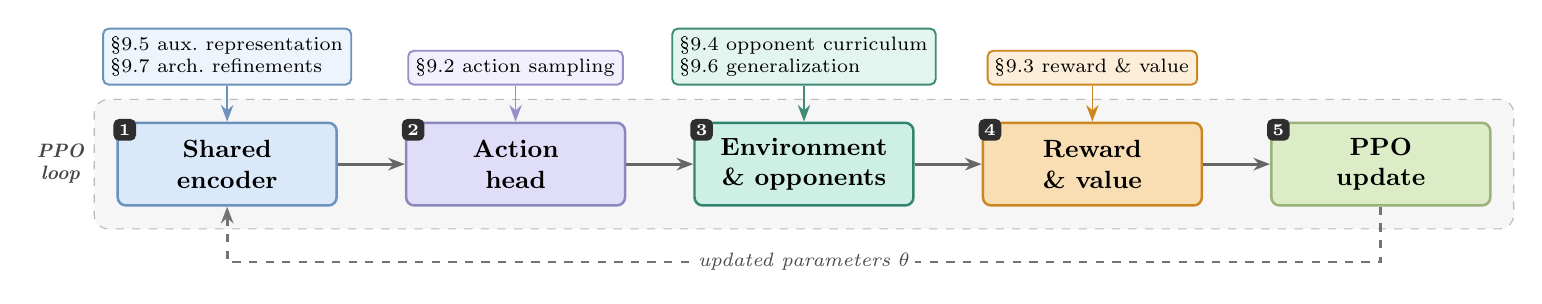
\begin{tikzpicture}[>={Stealth[length=6pt]}]

%% ── core PPO loop (data-flow order) ───────────────────────────────
\node[core, fill=encodercolor!30, draw=encodercolor!80!black] (encoder) {Shared\\encoder};
\node[core, fill=actorcolor!40,   draw=actorcolor!80!black,  right=0.85cm of encoder] (act) {Action\\head};
\node[core, fill=statecolor!30,   draw=envborder!85,          right=0.85cm of act]     (env) {Environment\\\& opponents};
\node[core, fill=rewcolor!35,     draw=rewcolor!85!black,     right=0.85cm of env]     (rew) {Reward\\\& value};
\node[core, fill=ppocolor!55,     draw=ppocolor!80!black,     right=0.85cm of rew]     (ppo) {PPO\\update};

%% ── black numbered stage pills (top-left corner of each box) ──────
\foreach \n/\stagename in {1/encoder, 2/act, 3/env, 4/rew, 5/ppo}
  \node[pill] at ([shift={(3pt,-3pt)}]\stagename.north west) {\n};

\draw[flow] (encoder) -- (act);
\draw[flow] (act) -- (env);
\draw[flow] (env) -- (rew);
\draw[flow] (rew) -- (ppo);

%% ── feedback: updated parameters flow back into the network ───────
\draw[->, line width=1pt, dashed, black!55, >={Stealth[length=6pt]}]
  (ppo.south) -- ++(0,-20pt) -| (encoder.south);
\node[font=\scriptsize\itshape, black!70, fill=white, inner sep=2pt]
  at ($(encoder.south)!0.5!(ppo.south)$) [yshift=-20pt]
  {updated parameters $\theta$};

%% ── subtle band behind the loop ──────────────────────────────────
\begin{pgfonlayer}{background}
  \node[draw=gray!55, dashed, rounded corners=5pt, inner sep=8pt,
        fill=gray!7, fit=(encoder)(act)(env)(rew)(ppo),
        label={[font=\scriptsize\itshape\bfseries, text=gray!55!black, align=center]left:{PPO\\loop}}]
        (loopframe) {};
\end{pgfonlayer}

%% ── section tags (raised above each stage) ───────────────────────
\node[tag, align=left, draw=encodercolor!80!black, line width=0.7pt, fill=encodercolor!15, above=13pt of encoder] (tenc)
  {\S9.5 aux.\ representation\\\S9.7 arch.\ refinements};
\node[tag, draw=actorcolor!85!black, line width=0.7pt, fill=actorcolor!18, above=13pt of act] (tact)
  {\S9.2 action sampling};
\node[tag, align=left, draw=envborder!80, line width=0.7pt, fill=statecolor!18, above=13pt of env] (tenv)
  {\S9.4 opponent curriculum\\\S9.6 generalization};
\node[tag, draw=rewcolor!85!black, line width=0.7pt, fill=rewcolor!18, above=13pt of rew] (trew)
  {\S9.3 reward \& value};

\draw[->, semithick, encodercolor!80!black] (tenc) -- (encoder);
\draw[->, semithick, actorcolor!85!black]   (tact) -- (act);
\draw[->, semithick, envborder!80]          (tenv) -- (env);
\draw[->, semithick, rewcolor!85!black]     (trew) -- (rew);

\end{tikzpicture}

\end{document}
